%!TeX encoding = UTF-8

%%%%%%%%%%%%%%%%%
% 不能在文章中使用中文
% 模板文档: http://mirror.aut.ac.nz/CTAN/macros/latex/contrib/apa6/apa6.pdf
% \section{我是一级标题} 一级标题
% \subsection{我是二级标题} 二级标题
% \subsubsection{我是三级标题} 三级标题
% 带括号引用 \parencite{文章简写}
%%%%%%%%%%%%%%%%%

%%%%%%%%%%%%%%%%%
% 文档定义
%%%%%%%%%%%%%%%%%
\documentclass[jou,a4paper]{apa6}
\usepackage[american]{babel}
\usepackage{csquotes}
\usepackage[style=apa,sortcites=true,sorting=nyt,backend=biber]{biblatex}
% 其他包
% 数学符号
\usepackage{amssymb}
% 导入csv表格
\usepackage{csvsimple}
% 导入图片
\usepackage{graphicx}
\graphicspath{ {./images/} }
% 超链接支持
\usepackage[hidelinks]{hyperref}
\DeclareLanguageMapping{american}{american-apa}
\addbibresource{bibliography.bib}

\title{CSFs in IT IMP: Project Management, Change Management and Risk Management}
% 页眉中的标题
\shorttitle{}

% 作者/组织
\twoauthors{Louis Lu}{Zhong Wei}
\twoaffiliations{Ara Institute of Canterbury}{Ara Institute of Canterbury}

\leftheader{}

% \abstract{}
% \keywords{}

%%%%%%%%%%%%%%%%%
% 文档正文
%%%%%%%%%%%%%%%%%
\begin{document}
% 隐藏页眉
% \thispagestyle{otherpage}
% 标题
\maketitle

%%%%%%%%%%%%%%%%%
% 目录
%%%%%%%%%%%%%%%%%
% \tableofcontents
% \clearpage

%!TEX root = ../assignment1.tex

\section{Introduction}

% 总起
In this article, we seek to identify critical success factors for IT projects by literature review, and then try to build an evaluation system to make an IT project successful. With that aim, we conduct a qualitative analysis to gather all the significant points of what the literature argue regarding this topic. A quantitative model is set up to select and prioritize the findings. The outcome of the model is a solution list. The aforementioned process will be done twice with respective resources, which results in an evaluation tool for researchers and practitioners to avoid similar failures in IT projects.

% 背景
\subsection{Background}
IT projects today tend to be agile, technical and complex\parencite[p. 2]{4} where pitfalls, issues and risks are everywhere in terms of time, people and budget. From a
project management perspective, the project was 193\% over schedule, 419\% over budget, and 130\% over scope\parencite[p. 8]{6}. A shockingly high failure rate also can be seen across some other publications in literature\parencite{2,3}.

% 背景中的三个关键词
\subsection{Keywords}
We investigate the literature and zoom in with the following keywords that influence success or failure of an IT project the most, which are project management, change management and risk management.

\paragraph{Project Management}
Project management is the planning to deliver the deliverables in a project, which academia believes, consists of 4-phase planning: initiating, planning, executing and controlling, while some researchers introduce the idea that this deliverable-targeted plan is considered as initiation, contagion, control and integration when a specific model in ERP projects is built\parencite[p. 3]{2}. Project management covers a lot of sub-areas such as time, scope, budget, quality, issues, risk and change. Success will be presented when a sophisticated project manager arrange them well in every stage.

\paragraph{Change Management}
Change management, as mentioned previously, is a sub-component of project management which researchers\parencite{3,6} have been putting emphasis on. In such an agile and technical and complex industry, the complexity of a project has inevitably made decision makers implement some changes for all or some stakeholders to transit to another new system\parencite[p. 1]{3} so that a better quality of the deliverables will be produced with the three constraints: scope, time, budget. The idea of change management has been regarded as a progressive method for attaining strong-minded conversion within a business or individuals sometimes\parencite[p. 3]{3}.

\paragraph{Risk Management}
Despite the fact that risk management is yet another sub-component of project management, a recent research by Bunker enlightens us by introducing disaster management from a change management perspective instead of a traditional project management perspective\parencite[p. 10]{6}. Intriguingly and similarly, the idea of emergent and scenario driven disaster management can be applied to the risk management.

% 文章结构
\subsection{Structure}
The article is divided into 7 sections: introduction, methodology, findings of Phase 1, findings of Phase 2, conclusion, summary and reflections. In introduction, a brief information is given, stating what we are investigating and what result we will produce. 3 aforementioned keywords are also introduced for future reference. The methodology describes how we conduct our research. A subsequent findings of Phase 1 will be presented with details using the defined method with data, where an evaluation is done. The findings of Phase 2 is structurally similar to the previous section, but with 10 case studies. In outcome, we will compare and contrast findings of both phases, then try to make an evaluation tool from our findings. The conclusion will revisit what we will have covered in previous sections. Summary will be provided as a briefing of the whole article. And eventually, there is a reflections section discussing the values and limitations of this research.

%!TEX root = ../assignment1.tex

\section{Methodology}
% 总流程
For this study, a qualitative analysis is first carried out, gathering all the possible solutions that the researchers suggest regarding success, failure and risks identified in project management, change management and risk management. All the 6 sources are in the reference list at end of the this article. They are from professional journals and forums published within 10 years from now. which reliability and professionalism can be assured.

% 列举文章和主题
In our selection of literature, \citetitle{1} and \citetitle{2} are on project management. \citetitle{3} is on change management while \citetitle{4} and \citetitle{5} are on risk management. \citetitle{6} gives an overview and an update of information system success and failure, which is composed by an affiliation of famous scholars in the field.

% 如何 coding
When utilizing the aforementioned selection of literature for qualitative analysis, we seek to identify issues, solutions and/or conclusions that authors have deduced or based on. Furthermore, the phases and the roles of stakeholders involved are also noted when a possible clues is identified. With the identified data, we reword the statements as possible proposals. All possible proposals with notation are what we have captured for subsequent evaluation process.

% 如何做 evaluation framework
With this captured data, an evaluation is processed where all the recommendation is listed and evaluated by how a given proposal affects on the phases of a project and on the roles of stakeholders in corresponding phases. To better employ the prioritized lists of proposals by some researchers who use statistical models, a cross-contextual coefficient is introduced during the evaluation process. In the evaluation process, global influence score of a proposal in a specific research context is calculated by the following formula \ref{brief}.
\begin{equation}
g_{C_{i},j} = \mathit{k_{C_{i},j}}l_{C_{i},j},\ C_{i,j} \in C_{i},\ C_{i} \in \mathbb{C}
\label{brief}
\end{equation}

In formula \ref{brief}, $\mathbb{C}$ denotes the set of all research contexts. And for each research context $C_{i}$ which is an element in $\mathbb{C}$, $C_{i,j}$ denotes a proposal in the given research context $C_{i}$. $g_{Ci,j}$ is the global influence score of a proposal in a given research context $C_{i}$. Similarly, $l_{C_{i},j}$ is the local influence score of the same proposal; $\mathit{k_{C_{i},j}}$ is the cross-contextual coefficient for the same proposal. Each element on the right hand side of the formula can be calculated respectively as follows.
\begin{equation}
\mathit{k_{C_{i},j}} = \frac{f_{C_{i,j}}}{\bar{f_{C_i}}}
\label{coefficient}
\end{equation}
\begin{equation}
\bar{f_{C_i}} = \frac{1}{n}\left (\sum_{m=1}^n{f_{C_{i,m}}}\right)
\label{mean}
\end{equation}
\begin{equation}
l_{C_{i},j} = |P_{C_{i,j}}||R_{C_{i,j}}|
\label{local_influence}
\end{equation}

In formula \ref{coefficient} and \ref{mean}, $f_{C_{i,j}}$ denotes the local influence score in a research context $C_{i}$ and $\bar{f_{C_i}}$ is the arithmetic mean value of all local influence scores of proposals in a given context $C_{i}$.

In formula \ref{local_influence}, $l_{C_{i},j}$ is the local influence score of a given proposal $C_{i,j}$. $|X|$ denotes the cardinality of the given set $X$. $P_{C_{i,j}}$ is the set of affected phases by the proposal $C_{i,j}$. Similarly, $R_{C_{i,j}}$ is that of affected roles of stakeholders in the same context.

Thus, the global influence score of a given proposal that denotes as $g_{C_{i},j}$ can be calculated as follows:
\begin{equation}
g_{C_{i},j} =
\frac
% 分子 k local=(P R)
{f_{C_{i,j}} |P_{C_{i,j}}| |R_{C_{i,j}}|} 
% ----分式线-----
% 分母 f平均
{\frac{1}{n}\left (\sum_{m=1}^n{f_{C_{i,m}}}\right)}
% 满足条件
,\ 
C_{i,j} \in C_{i},\ C_{i} \in \mathbb{C}
\label{final}
\end{equation}

An higher score of $g_{C_{i},j}$ indicates that the proposal has a wider and deeper influence on project success. We post-process the result of score by descending ranking, in which we select the ones higher than average value. This subset of proposals are tagged by sub-topics and enrolled in a checklist as solutions.

%!TEX root = ../assignment1.tex

\section{Findings of Phase 1}

\subsection{Overview Of Data}
In our selection of literature, 6 articles are employed. \citetitle{1} and \citetitle{2} are on project management. \citetitle{3} argues about change management while \citetitle{4} and \citetitle{5} are on risk management. \citetitle{6} gives an overview and an update of information system success and failure, which is composed by an affiliation of famous scholars in the field.

\subsection{Gaps and Solutions}

The gaps and the solutions often express the same meanings but with different wording. Gaps are often stated as "lack of something" while the solutions suggest to supplement the missing part. Therefore, we only collect the proposals that the literature suggests, for the sake of conciseness.

We have extracted 32 sections containing 48 proposals contributing to success, failure or risks from the 6 articles. We have also tagged the affected phases and the affected roles for each proposal. The weights of priority are also recored and normalized in the researches where the authors conclude with a math model. A baseline value of $1$ is given to those proposals from which the authors have not built a math model.

Using the aforementioned primary themes, regarding the 4 main themes, that is control, process, people and structurehere, we have got many findings below:

\subsubsection{Samples: Control}

On page 9 of \citetitle{3}, \citeauthor{3} argue that the design must be established consistently.

\begin{quotation}
Obviously, to prevent unnecessary reconfiguration at each implementation stage, a consistent well-thought-out ERP design that meets the needs of the organization should be established.
\end{quotation}

On page 11 of \citetitle{2}, \citeauthor{2} put emphasis on the suggestion that proactively assess performance of vendor and develop a list of performance metrics for vendors.

\begin{quotation}
  The project manager should set up objective and clear evaluation criteria for the supplier in advance and ensure that the supplier complies with the evaluation criteria during the implementation of the project. In addition, the project manager should regularly evaluate the progress of the project rather than just evaluating it at the end of the project. Only in this way, once the deviation from the standard occurs, the project manager can know what and why the deviation occurs in time, and take appropriately measures to ensure that the deviation is solved in time. After all, it is not enough to rely solely on the vendor to solve problems themselves. In general, periodically assessment is important because it is a reliable method to help the project manager understanding the situation of that time. Additionly, it is also good to maintain a good vendor-client partnership.
\end{quotation}

\subsubsection{Samples: Process}
\citeauthor{2} suggests that keep 85\% of business process common and setup a decision committee on page 11 of \citetitle{2}.

\begin{quotation}
  To establish and maintain better relationship between project managers and the management, on the one hand, project manages should keep the project scope as consistent as possible with the management; on the other hand, in order to reduce or avoid the resistance of end users from different regions, product managers should consider forming a priority committee. It can be an important scope management tool because its members come from different regions, so the scope decision process is largely transparent to them.
\end{quotation}

\citeauthor{6} recommend that it is better to identify the problem before proposing a solution, and to understand user requirements before designing a system on page 10 of \citetitle{6}.

\begin{quotation}
A common mistake is to start designing a solution only with a rough understanding of the problem to be solved, especially for those experienced people. As the saying goes, a good question is better than a great answer. It can be a essential rule that taking more time to understand the problem before making a decision. (Bergman et al. 2002)
\end{quotation}

\subsubsection{Samples: People}
In \citetitle{3}, the author argue that it is important to have effective communication at each level.

\begin{quotation}
Efficient and effective communication is an integral part of the successful implementation of IT projects. During an IT project life cycle, communication is neccessary at every level of the project. According to Mandal and Gunasekaran (2003), opinions from users about their requests, responses, objections or approvals are always important. Project progress should be communicated regularly to management so they can understand the current status of the project. As for the objectives, activities, news or udpates, it should be promptly notified to the relevant staff in the project.
\end{quotation}


To manage the communication process and create a forum is the suggestion given by \citeauthor{2} when talking about success of building an ERP system.

\begin{quotation}
Therefore, the project manager should work hard to manage the communication process, including communicating with management and communicating downwards. Based on this, it is necessary to create a forum where stakeholders can prioritize and discuss issues. There are various conflicts between business and IT projects, and successfully managing these conflicts is essential to the success of IT projects. Guiding end-users to participate in projects can effectively reduce or resolve these conflicts, and those projects that end users actively participate in are often successful.
\end{quotation}


\subsubsection{Samples: Structure}
\citeauthor{6} believe that getting top management support is important for the successful implementation of IT on page 10 of \citetitle{6}
\begin{quotation}
First, it is important to get top management support. This is probably the most common injunction for the successful implementation of IT in both the IS research and practitioner literature. This injunction has been given for more than three decades (Markus 1983) and continues to be given today (Elbanna 2012).
\end{quotation}

For vendor support, \citeauthor{6} also suggest that it is important to obtain “independent” advice from a consultant.
\begin{quotation}
Fifth, in order to compare the claims of various vendors appropriately, it is a good idea to obtain “independent” advice from a consultant (Pollock and Williams 2009).
\end{quotation}

\subsection{Evaluation Of Solutions}
To clarify the result, we collect the data into a spreadsheet in which contains the following criteria: No., proposal, article identifier, coding identifier, affected phases, affected roles.
% \begin{table}[ht] 
% \caption{Coding(header only)}
% \resizebox{\columnwidth}{!}{%
% \csvautotabular{tables/coding_sample.csv}
% }
% \label{tab:sample}
% \end{table}

With the defined method, we tag our research contexts in the following sequence.
$C_{1}$ is \citetitle{1}.
$C_{2}$ is \citetitle{2}.
$C_{3}$ is \citetitle{3}.
$C_{4}$ is \citetitle{4}.
$C_{5}$ is \citetitle{5}.

According to the defined method, we have everything for the evaluation process. Due to the fact that the studies are not conducted with a math model in $C_{2}$ and $C_{4}$, we assume all the solutions from aforementioned researches are of equal importance. Therefore, we pad the cross-contextual coefficient with a baseline value of 1 to $\mathit{f_{C_{2,j}}}$ and $\mathit{f_{C_{4,j}}}$.

Using the formula \ref{final}, we calculate the global influence score for each proposal. Here is a visualization of the scores of all the proposals.

\begin{figure}[ht]
\centering
\resizebox{\columnwidth}{!}{%
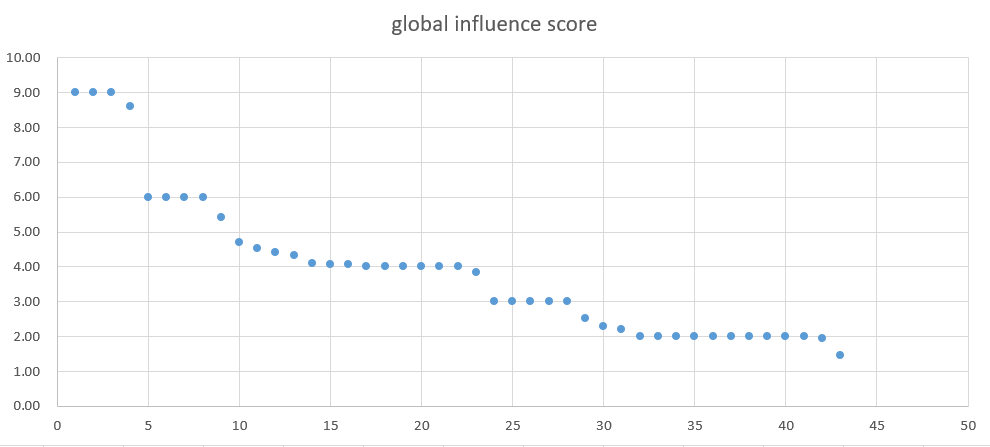
\includegraphics{global_influence_score.png}
}
\end{figure}

In the plot, the horizontal axis stands for all the proposals in context $\mathbb{C}$ and the vertical axis for global influence score. It is clear that there are 4 proposals of significant influence clustering at the top followed by a second group at range roughly between 4 to 6. The trailing group of low influence score occupies the range between 1 to 3.

\subsection{Result Of Evaluation}
For the effectiveness and conciseness, we truncate the trailing group scored lower than average($\bar{g}=3.60$), which is also the trailing group. We obtain the following list of solutions.

\begin{table}[ht]
\caption{Solution List}
\resizebox{\columnwidth}{!}{%
\csvautotabular{tables/solutions.csv}
}
\label{tab:solution}
\end{table}

% To track their origins of sources, we mark them with the article themes as shown in \ref{tab:solution}. There are 10 solutions about project management, 8 about risk management and 5 about change management.

%!TEX root = ../assignment1.tex

\section{Findings Of Phase 2}

\subsection{Overview Of Data}
In Phase 2, 10 case studies are given on how projects failed in Victoria Australia. The cases are government related information communication and technology projects. The author\parencite{case_study} provides well structured anatomy of projects where issues are discussed in depth by topics. Additionally, some recommendations are given by the author, some of which are responded by the project owners.

\subsection{Gaps and Solutions}
Using the same method, we collect gaps and possible solutions(proposals) for further evaluation. There are 54 sections of gaps reflecting 54 proposals to 10 case studies. The author uses no mathematical model to prioritize gaps, a baseline value of $1$ is also used to all the proposals, according to the predefined methodology.

The collected data are tagged with the same four themes: control, process, people and structure. Here are some samples under each theme.

\subsubsection{Samples: Control}
% id 21
In case 4, the author argues that the longer planning that spans in time, the more risk of redesigned. Ultimately, project will be likely to fail due to this uncertainty of change. In initial phase of project, project leaders should plan funding well in initial phase with top management support.
\begin{quotation}
The longer it takes to fund the project, the longer it will take for the outdated systems to be replaced, the more likely it is the costs will be increased and the more likely it is that the project will need to be redesigned.
\end{quotation}


% id 2
In case 1, it is the rushing to meet deadlines that fails to deliver design goals. For cover-up, benefits are altered to please government. Project managers should define measurement of deliverables and change accordingly. 
\begin{quotation}
The business case was rushed to meet budget timelines and to fit within the funding already allocated by the government. It failed to identify measurable benefits. Instead, benefits were written to obtain government support.
\end{quotation}

\subsubsection{Samples: Process}
% id 26
poor user training and post-implementation support result in bad experience among users. Better user training and support should be designed and implemented in early stage of project planning.

\begin{quotation}
Despite being introduced in July 2008, CRIS continues to suffer from inadequate training, poor help-desk support, and slow responses to functionality change requests.
\end{quotation}

% 30
training cost is not included in the planning process. It is suggested to consider training in cost planning.
\begin{quotation}
Training costs have not been fully calculated or recorded against the project. The original business case indicated training would  cost \$23 million.
\end{quotation}

\subsubsection{Samples: People}
% 34
failing to detect risk of vendor results in bad contract deals. Vendor support should be reviewed by a third party in planning.
\begin{quotation}
A change in vendor ownership and concerns of vendor withdrawal led to DOJ making contractual concessions.
\end{quotation}

% 37
project fails and leads to alternative solution when requirements are not communicated precisely. It is import to understand requirements and define deliverables between project manager and users.
\begin{quotation}
According to the Supreme Court, ICMS’s case management system (CourtView) fails to meet the court’s needs. The Supreme Court has ultimately resolved to pilot its own system to provide case management.
\end{quotation}

\subsubsection{Samples: Structure}
% 4
The vacancy of a project leader results management chaos. It is important to have a project leader.
\begin{quotation}
Victoria Police failed to appoint a single, qualified project manager to run the project, notwithstanding that project management was identified as a project risk in the business case and a major contributor to the failure of 60-70 per cent of ICT-related projects.
\end{quotation}

% 19
The organization structure stops from making a timely funding to implement the project. A better organization is advised.
\begin{quotation}
The government approved VicRoads spending \$52 million on RandL over three years while the Cabinet budget committee was apparently uncertain about the project and there was a risk that the project would not receive the required funding. This risk eventuated.
\end{quotation}
\subsection{Evaluation Of Solutions}

\subsection{Result Of Evaluation}
%!TEX root = ../assignment1.tex

\section{Comparision}

%!TEX root = ../assignment1.tex

\section{Conclusion}


%!TEX root = ../assignment1.tex

\section{Section}

%!TEX root = ../assignment1.tex


%%%%%%%%%%%%%%%%%
% 参考文献
%%%%%%%%%%%%%%%%%
\printbibliography
\end{document}
